\documentclass{article}

\usepackage{graphicx}
\usepackage{algorithm}
\usepackage{algpseudocode}
\usepackage{authblk}
\usepackage{url}
\usepackage[utf8]{inputenc}
\usepackage{color}
\usepackage{amsmath}
\graphicspath{{C:\Users\tkhal\Desktop\College\Second Yr\Data Analysis EE201\Project\Question 2}}

\title{AI Assignment-1 Report}
\vspace{20pt}
\vspace{20pt}
\date{\today}
\author{Team -14 \\Tabish Khalid Halim , \\ 200020049 \\ Anand Hegde , \\ 200020007}
\vspace{20pt}
\affil{Department of Computer Science, IIT Dharwad}
\begin{document}

\maketitle
\pagenumbering{gobble}
\newpage
\tableofcontents

\newpage
\pagenumbering{arabic}
\section{Approach}
The basic approach we used for the A.I assignment is to use the concept of graphs \& vertices and 
applied BFS\{Breadth First Search\} , DFS \{Depth First Search\} and DFID \{Depth First Iterative Deepening Search\}.
\vspace{10pt}
\\
Along with applying the above algorithms for the PacMan , we have also set the preference order for adding the neighbor nodes which are:
\\$$DOWN > UP > RIGHT > LEFT$$
\vspace{10pt}
\\If the input number $\in \{0,1,2\}$ , then the program executes the algorithms BFS , DFS and DFID respectively .
\vspace{10pt}
\\After visiting the neighbors in the maze graph, We can easily find out the length of the path and the number of states for the maze.
\newpage
\section{Variables used in Python Program}
\vspace{20pt}
\begin{itemize}
    \item \textbf{dfs\_stop} : tells when dfs to stop.
    \item \textbf{goaldfs} : target state to achieve for DFS.
    \item \textbf{goaldfid} : target state to achieve for DFID.
    \item \textbf{statesdfs} : No. of states explored during DFS traversal .
    \item \textbf{statesdfid} : No. of states explored during DFID traversal .
    \item \textbf{DFIDstop} : to break out of recursion .
    \item \textbf{visited} :  Variable created to store the set of visited vertices .
    \item \textbf{parent} : Tuple to store the parent of each node . It is used for finding path .
    \item \textbf{graph\_input} :  This stores the input given in as a list of lists .
    \item \textbf{m} : No. of rows in the Maze .
    \item \textbf{n} : No. of columns in the Maze .
    \item \textbf{states} : Variable to store no. of states explored .
    \item \textbf{pathlength} : Variable to store length of the path .
\end{itemize}
\newpage
\section{Functions created in Python Program}
\vspace{20pt}
\begin{itemize}
    \item \textbf{goal\_state(i,j,graph\_input)} : This function determines whether the coordinate (i,j) is the end goal for the PacMan or not .
    \item \textbf{move\_gen(i,j,graph\_input)} : This function's task is returning all \\possible moves available to the PacMan
    , if the adjecent block has a space\\(' ') or astrik('*') 
    , funtion returns its coordinates .
    \item \textbf{DFSUtil(v, visited,parent,graph\_input,open\_list)} : This is the recursive DFS Utility function .
    \item \textbf{DFS(graph\_input,v=(0,0))} : The function to do DFS traversal. It uses recursive DFSUtil()- dfs utility function .
    \item \textbf{DFID(graph\_input, depth,v=(0,0))} : The function to do DFID traversal. It uses recursive DFSUtil()- DFS Utility Function.
    \item \textbf{DFIDUtil(v, visited,parent,graph\_input, depth)} : This is recursive DFID- utility function .
    \item \textbf{dfid(graph\_input,v=(0,0))} :  This is the Main DFID function- which calls DFID- which is dfs version for DFID . The extra thing is the depth here.
    \item \textbf{bfs(graph\_input,s=(0,0))} : This function is used to perform BFS .
    \item \textbf{searchmethod(bdd,graph\_input)} : Simple function to deal with the case wise operation to perform BFS, DFS or DFID as per the requirement
\end{itemize}
\newpage
\section{Pseudo Code}
The main pseudo code used in our assignment is as follows :
\subsection*{move\_gen function}
\vspace{5pt}
def move\_gen(i,j,graph\_input):
\vspace{5pt}
    \\ \hspace*{20pt}global open\_list
    \vspace{2pt}
    \\ \hspace*{20pt}templist=[]
    \vspace{2pt}
    \\ \hspace*{20pt}if(i$<$n-1):
    \vspace{2pt}
    \\ \hspace*{30pt}    if((graph\_input[i+1][j]==' ' or '*') and ((i+1 , j) not in open\_list)):
    \vspace{2pt}
    \\ \hspace*{40pt}        templist.append((i+1 , j))
    \vspace{2pt}
    \\ \hspace*{20pt} if(i$>$0):
    \vspace{2pt}
    \\ \hspace*{30pt}    if(graph\_input[i-1][j]==' ' or '*') and ((i-1 , j) not in open\_list):
    \vspace{2pt}
    \\ \hspace*{30pt}        templist.append((i-1,j))
    \vspace{2pt}
    \\ \hspace*{20pt} if(j$<$n-1):
    \vspace{2pt}
    \\ \hspace*{30pt}    if(graph\_input[i][j+1]==' ' or '*') and ((i , j+1) not in open\_list):
    \vspace{2pt}
    \\ \hspace*{40pt}        templist.append((i,j+1))
    \vspace{2pt}
    \\ \hspace*{20pt} if(j$>$0):
    \vspace{2pt}
    \\ \hspace*{30pt}    if(graph\_input[i][j-1]==' ' or '*') and ((i+1 , j) not in open\_list):
    \vspace{2pt}
    \\ \hspace*{40pt}        templist.append((i,j-1))
    \vspace{2pt}
    \\ \hspace*{20pt}return templist
\subsection*{goal\_state function}
    \vspace{5pt}
    def goal\_state(i,j,graph\_input):
    \vspace{5pt}
        \\ \hspace*{20pt}if(graph\_input[i][j]=='*')
        \vspace{5pt}
        \\ \hspace*{30pt} return True
        \vspace{2pt}
        \\ \hspace*{20pt}else :
        \vspace{5pt}
        \\ \hspace*{30pt} return True
\newpage
\section{Graphical Analysis}
\vspace{5pt}
Based on observation , we have plotted the following time vs size of maze graph for BFS and DFS .
\vspace{20pt}
\\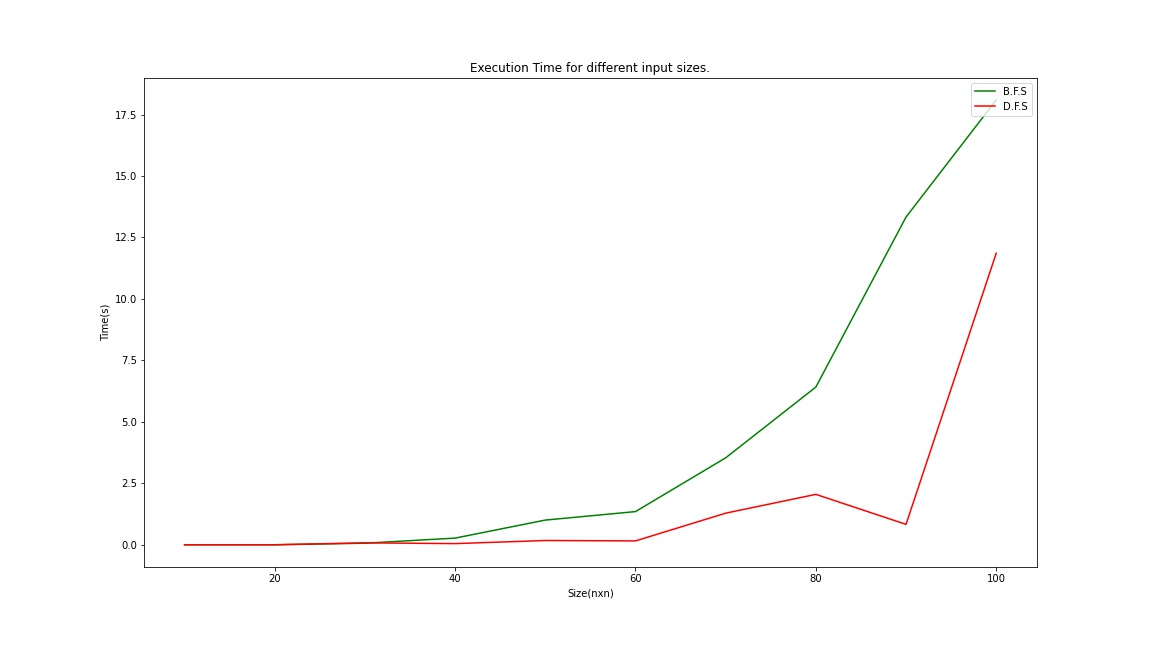
\includegraphics[scale=0.3]{time.jpg}
\\By far , we have observed that DFID is the slowest initially but potentially more better for bigger mazes .
\vspace{20pt}
\\Here is the following table depicting the dependence of no. of states and path length on priority order [U : Up, D : Down , R : Right, L :Left].
\vspace{10pt}
\\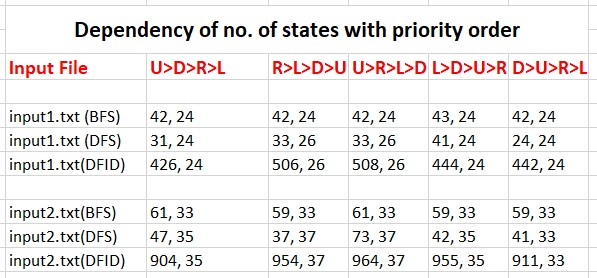
\includegraphics{table.jpg}
\newpage
\section{Results}
\vspace{20pt}
The following conclusions have been made after evaluation of my program : 
\begin{enumerate}
    \item The Output for the first test case :
    \\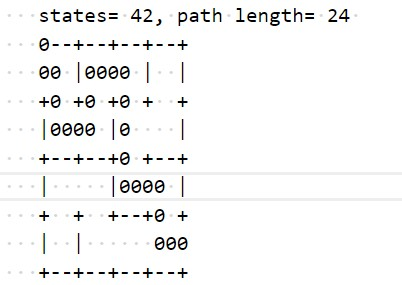
\includegraphics{Output1.jpg}
    \item The Output for the second test case :
    \\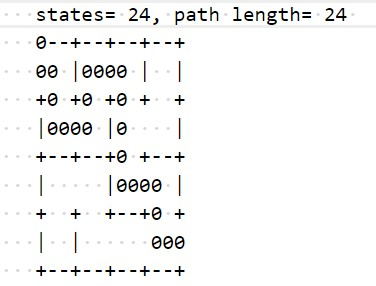
\includegraphics{Output2.jpg}
\newpage
    \item The Output for the third test case :
    \\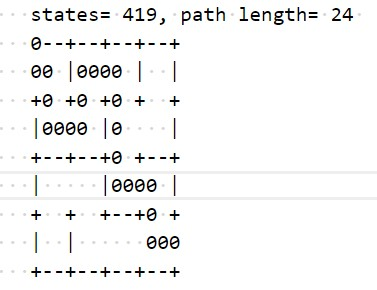
\includegraphics{Output3.jpg}
    \item The Output for the fourth test case :
    \\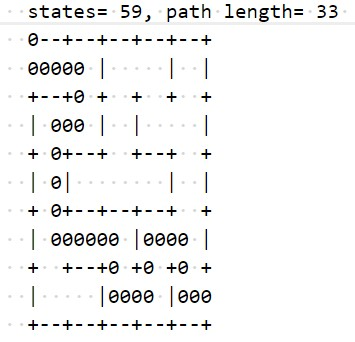
\includegraphics{Output4.jpg}
\newpage
    \item The Output for the fifth test case :
    \\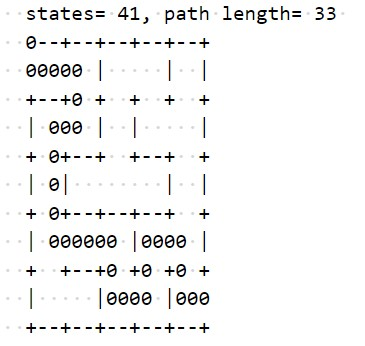
\includegraphics{Output5.jpg}
    \item The Output for the sixth test case :
    \\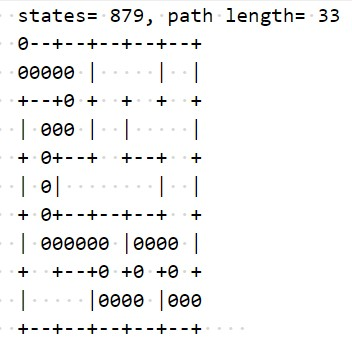
\includegraphics{Output6.jpg}
\end{enumerate}
\vspace{20pt}
\subsection*{Conclusion}
\textbf{Thus , BFS, DFS and DFID algorithms which are uninformed search methods always gives the solution to the problem , but it might not be optimal in every case .}
\newpage
\section{References}
\vspace{30pt}
\begin{itemize}
    \item \url{http://geeksforgeeks.com}
    \item \url{https://wikipedia.org}
    \item \url{https://stackoverflow.com}
    \item \url{http://www.delorie.com/game-room/mazes/genmaze.cgi}
\end{itemize}
\end{document}